\documentclass[12pt]{article}
\usepackage[english]{babel}
\usepackage{natbib}
\usepackage{url}
\usepackage[utf8x]{inputenc}
\usepackage{amsmath}
\usepackage{graphicx}
\graphicspath{{images/}}
\usepackage{parskip}
\usepackage{fancyhdr}
\usepackage{lastpage}
\usepackage{vmargin}
\usepackage{hyperref}
\usepackage{float}

\usepackage{alltt}
\usepackage{tcolorbox}
\newtcolorbox{mybox}{top=1mm, bottom=1mm, left=1mm,right=1mm, boxsep=0mm, width=1\linewidth, breakable, enhanced, opacityframe=0.2, arc=0mm}
\usepackage{listings}
\usepackage{pgfkeys}
\tcbuselibrary{breakable, fitting}
\tcbuselibrary{skins}
\tcbset{skin=enhanced}

\usepackage{color}
\definecolor{mygreen}{rgb}{0,0.6,0}
\definecolor{mygray}{rgb}{0.5,0.5,0.5}
\definecolor{mymauve}{rgb}{0.58,0,0.82}
\definecolor{codegreen}{rgb}{0,0.6,0}
\definecolor{codeorange}{rgb}{1.0,0.3,0}
\definecolor{codegray}{rgb}{0.3,0.3,0.3}
\definecolor{codepurple}{rgb}{0.58,0,0.82}
\definecolor{backcolour}{rgb}{0.96,0.96,0.96}

\usepackage{listings}
\usepackage[T1]{fontenc}
% macro to select a scaled-down version of Bera Mono (for instance)
\makeatletter
\newcommand\BeraMonottfamily{%
  \def\fvm@Scale{0.8}% scales the font down
  \fontfamily{fvm}\selectfont% selects the Bera Mono font
}
\makeatother
\lstdefinestyle{mystyle}{
    backgroundcolor=\color{backcolour},   
    commentstyle=\color{codegray},
    keywordstyle=\color{codegreen},
    numberstyle=\tiny\color{codegray},
    stringstyle=\color{codeorange},
    basicstyle=\BeraMonottfamily, 
    breakatwhitespace=false,         
    breaklines=true,                 
    captionpos=b,                    
    keepspaces=true,                 
    numbers=left,                    
    numbersep=5pt,                  
    showspaces=false,                
    showstringspaces=false,
    showtabs=false,                  
    tabsize=2
}
\lstset{style=mystyle}

\setmarginsrb{3 cm}{2.5 cm}{3 cm}{2.5 cm}{1 cm}{1.5 cm}{1 cm}{1.5 cm}

\title{Distributed TensorFlow \\[10pt] {\LARGE A performance evaluation}}								% Title
\author{Emanuele Bugliarello}								% Author
\date{12 Sept 2015}											% Date

\makeatletter
\let\thetitle\@title
\let\theauthor\@author
\let\thedate\@date
\makeatother

\pagestyle{fancy}
\fancyhf{}
\rhead{Page~\thepage~of~\pageref{LastPage}}
\lhead{\textit{Distributed TensorFlow: A performance evaluation}}
% \cfoot{\thepage}

\begin{document}

%%%%%%%%%%%%%%%%%%%%%%%%%%%%%%%%%%%%%%%%%%%%%%%%%%%%%%%%%%%%%%%%%%%%%%%%%%%%%%%%%%%%%%%%%

\begin{titlepage}
	\centering
%     \vspace*{-2 cm}
    
\includegraphics[scale = 0.5]{logocscs.png}\hfill
\includegraphics[scale = 0.85]{logoethz.png}\\[2.0 cm]	% University Logo
    
	\rule{\linewidth}{0.4 mm} \\[0.4 cm]
	{ \huge \bfseries \thetitle}\\[0.4 cm]
	\rule{\linewidth}{0.4 mm} \\[0.5 cm]
    
    \textsc{\LARGE \theauthor}\\[0.25 cm]
    {\large\texttt{emanuele.bugliarello@gmail.com}}\\[2.0 cm]	% University Name

	\textsc{\Large Summer Internship Report}\\[0.5 cm]	% University Name

    \textsc{\Large \today}\\[3.0 cm]				% Course Code
    
	\begin{flushleft} \large
		\emph{Supervisors:}\\
		Marcel Schöngens\\
        Maxime Martinasso\\
        Claudio Gheller\\
    \end{flushleft}
	
\end{titlepage}

%%%%%%%%%%%%%%%%%%%%%%%%%%%%%%%%%%%%%%%%%%%%%%%%%%%%%%%%%%%%%%%%%%%%%%%%%%%%%%%%%%%%%%%%%

\tableofcontents
\pagebreak

%%%%%%%%%%%%%%%%%%%%%%%%%%%%%%%%%%%%%%%%%%%%%%%%%%%%%%%%%%%%%%%%%%%%%%%%%%%%%%%%%%%%%%%%%

\section{Introduction}
In the past few years, deep neural networks have made breakthroughs in a wide variety of everyday technologies, such as speech-recognition on our smartphones, machine translation and in image recognition.
The success of deep learning is built upon the availability of a vast volume of data and as their sizes grow larger, it can take weeks to train deeper neural networks to the desired accuracy.
Fortunately, we are not restricted to a single machine and research has been conducted on enabling efficient distributed training of neural networks.\\

There are dozens of open source machine learning libraries that can be used to develop deep learning applications.
Here, we focus on TensorFlow, Google's open source machine learning framework.
There are two main reasons why we analyze TensorFlow: first, TensorFlow offers a flexible architecture allows you to deploy computation to one or more CPUs or GPUs in a desktop, server, or mobile device with a single API.
Second, most CSCS clients use TensorFlow as their deep learning framework.\\

In this report, we analyze the performance of distributed training in TensorFlow (in terms of number of images trained per second) in different systems and compare our results with the benchmarks available in TensorFlow's website.\\

The remainder of this report is organized as follows. 
We first give a brief overview of TensorFlow, present its architecture in distributed training and explain how to easily extend existing single-machine code to run on multiple nodes.
We then introduce the systems on which we will run our benchmarks and give some pointers on how to set them up.
Next, we describe the scripts we have written to easily run TensorFlow in a distributed environment, with a focus on Piz Daint which runs with Slurm Workload Manager.
A case study on MNIST is presented to show how to extend a single-node TensorFlow application to run across multiple nodes.
After that, we detail our methodology and discuss the results that we obtain when scaling out to 128 GPUs.
Finally, we present directions for future work and conclude this report.
\newpage

\section{TensorFlow}
TensorFlow~\cite{tf} is an open source software library for numerical computation using data flow graphs.
Nodes in these graphs represent mathematical operations, while multidimensional arrays (tensors) move across the edges between them; hence the name.
An example of a computational graph is shown in Figure \ref{fig:comp-graph}.
\begin{figure}[H]
  \centering
  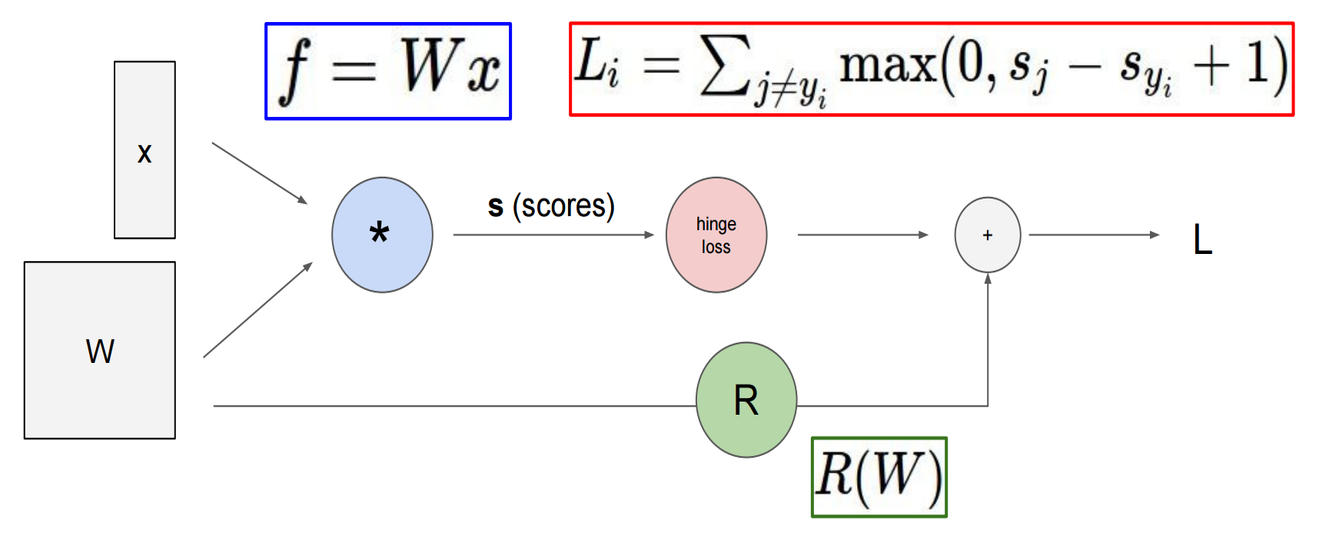
\includegraphics[width=0.8\textwidth]{comp-graph}
  \caption{Computational graph for a regularized Multiclass SVM loss \cite{deepsw}.} 
  \label{fig:comp-graph}
\end{figure}

In TensorFlow, you firstly build the computational graph and then run instances of that graph.
By doing so, the graph is created only once and the framework can apply some optimizations for you before it runs.\\

To make this more concrete, let's consider the linear regression example described in Figure \ref{fig:lin_reg-graph}. 
The corresponding TensorFlow code is shown in Listing \ref{listing:lin-reg}.
\begin{figure}[H]
  \centering
  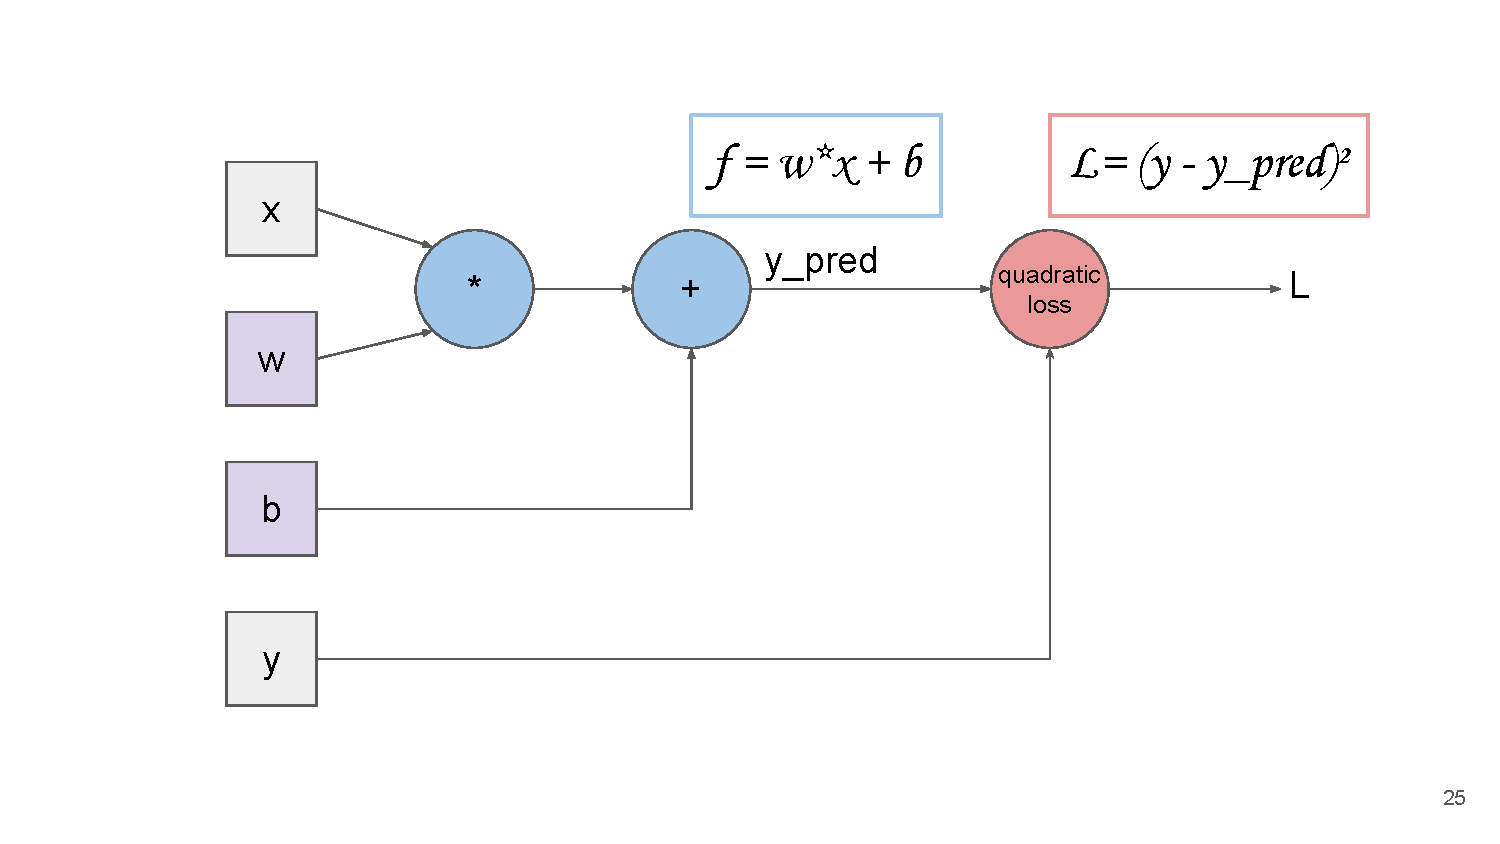
\includegraphics[width=0.75\textwidth, trim={3.5cm 2.2cm 2.2cm 1.8cm}, clip]{simple-graph.pdf}
  \caption{Linear regression computational graph.} 
  \label{fig:lin_reg-graph}
\end{figure}

\lstinputlisting[label=listing:lin-reg, language=Python, caption=Linear regression in TensorFlow., firstline=5,lastline=56]{listings/linear_reg.py}

In the previous snippet, when we build the data flow graph, every variable (such as \texttt{x}, \texttt{w}, \texttt{loss}, and \texttt{train}) is not assigned any value but it is actually an \textit{operation} that is added to the graph.
Specifically, a \texttt{tf.placeholder} represents a container for future values that will be loaded at run time, a \texttt{tf.Variable} instead represents a tensor that will be modified by the learning algorithm during the optimization phase, while the other ones are mathematical operations, as shown in Figure \ref{fig:lin_reg-graph}.\\

We start an execution by opening a \texttt{tf.Session}, to which we pass the graph defined before.
Here, we firstly initialize our \texttt{tf.Variable}s by assigning them their initial value, and then train our model for $\texttt{N\_EPOCHS}$ epochs~\footnote{An epoch is one complete presentation of the training data set to a machine learning model.} by passing each time an input and an output sample via $\texttt{feed\_dict}$ in \texttt{sess.run()}.
\texttt{sess.run()} evaluates the list of operations that are passed in its first argument.
It does so by computing only the nodes in the graph these operations depend on and returns their values at the end of the evaluation.\\

The resulting linear model is shown in Figure \ref{fig:lin_reg-plot}.
\vfill
\begin{figure}[t]
  \centering
  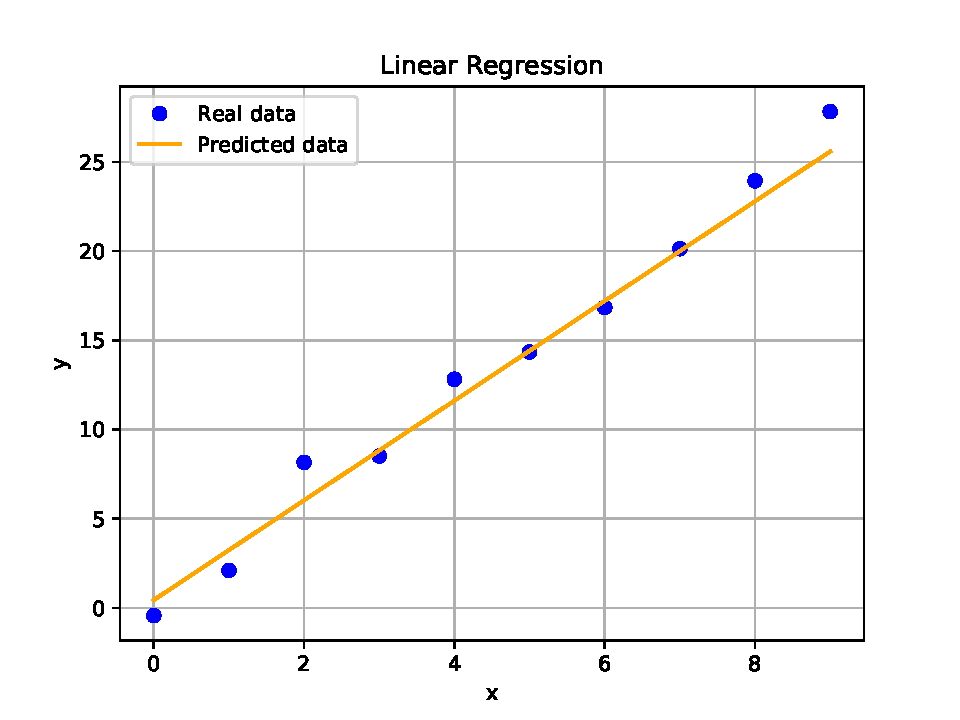
\includegraphics[width=0.7\textwidth,trim={0.5cm 0cm 0cm 0.5cm},clip]{linear_reg.pdf}
  \vspace{-0.5cm}
  \caption{Linear model learned with the example code in Listing \ref{listing:lin-reg}.}
  \label{fig:lin_reg-plot}
\end{figure}

% \begin{mybox}
% 	\begin{center}
% 	\begin{alltt}\tcbfontsize{0.9}
% 	lspci -k | grep -A 3 -i "network"
% 	\end{alltt}
% 	\end{center}
% \end{mybox}
% \noindent


\subsection{Distributed training} \label{sec:tf-dist-th}

As neural networks become larger, it can take weeks to train one of them to achieve the desired accuracy.
It is then of primary importance to distribute the training of these deep neural networks at a massive scale and reduce the training time to hours.\\
TensorFlow offers a large degree of flexibility in the placement of graph operations, allowing easy implementations for parallel computation across multiple workers.\\[-0.2cm]

When splitting the training of a neural network across multiple nodes, the most common strategy is data parallelism, where each node has an instance of the model and reads different training samples.\\
When using TensorFlow, this is achieved with the so-called ``between-graph replication'' setting.
In this context, processes have one of two roles: \textit{Parameter Servers (PS)} or \textit{Workers}.
The former ones host the trainable variables and update them with the values sent by the Workers.
Workers, on the other hand, run the model, send their local gradients to the PSs and receive the updated variables back.\\[-0.2cm]

In doing so, it is essential that all the Workers send their updates of each variable to the same PSs.
To ensure correct device placement of each variable, TensorFlow offers $\texttt{replica\_device\_setter}$, which provides a deterministic method for variable allocation, ensuring that the variables reside on the same devices.\\

Given that each Worker runs the same model, the only high-level changes required in a parallel implementation are the definition of the cluster of nodes and the role of each of them (Parameter Server/Worker).
The following code snippet (from \cite{dist_tf_intro}) shows how to specify such configuration in TensorFlow.
Note that such a script would be executed on each machine in the cluster, but with different arguments.

\begin{lstlisting}[label=listing:tfdist, language=Python, caption=Distributed TensorFlow skeleton.]
import sys
import tensorflow as tf

# Specify the cluster's architecture
cluster = tf.train.ClusterSpec({'ps': ['192.168.1.1:1111'],
                                'worker': ['192.168.1.2:1111',
                                           '192.168.1.3:1111']
                               })

# Parse command-line to specify machine
job_type = sys.argv[1]  # job type: "worker" or "ps"
task_idx = sys.argv[2]  # index job in the worker or ps list
                        # as defined in the ClusterSpec

# Create TensorFlow Server. This is how the machines communicate.
server = tf.train.Server(cluster, job_name=job_type, task_index=task_idx)

# Parameter server is updated by remote clients.
# Will not proceed beyond this if statement.
if job_type == 'ps':
  server.join()
else:
  # Workers only
  with tf.device(tf.train.replica_device_setter(
                      worker_device='/job:worker/task:'+task_idx,
                      cluster=cluster)):
    # Build your model here as if you only were using a single machine

  with tf.Session(server.target):
    # Train your model here
\end{lstlisting}

The first step in running distributed TensorFlow is to define the architecture of the cluster using \texttt{tf.train.ClusterSpec}, where the IP addresses and ports of all the processes for each role are provided.\\
% 
Next, the script determines its job type (or role) and its index among all the processes with the same job type.
This is typically achieved by passing command-line arguments to the script, which are then parsed. 
Here, $\texttt{job\_type}$ specifies whether the node is running a Parameter Server or a Worker task, whereas $\texttt{task\_idx}$ specifies the process's index into its task list. 
An important remark regarding $\texttt{task\_idx}$ is that the list of nodes per role is interpreted as a sorted array.
That is, you cannot arbitrarily set the $\texttt{task\_idx}$ of a given process; instead, this must reflect the position of that process in the original PS or Worker list specified in \texttt{tf.train.ClusterSpec}.
For instance, the script for Worker \texttt{192.168.1.2:1111} must be launched setting its $\texttt{task\_idx}$ to $0$ as it is the first Worker in the list.\\[-0.2cm]

The next step is to use this information to create a TensorFlow Server, which allows this process to communicate with any other server in the same cluster and participate in distributed training.\\[-0.2cm]

If the node is a Parameter Server, it simply joins its threads and waits for them to terminate. 
While it may seem counterintuitive that there is no PS-specific code, the graph elements are actually pushed to it from the workers.\\[-0.2cm]

Conversely, if the device is a Worker, we use $\texttt{replica\_device\_setter}$ to build our model, so that parameters are consistently allocated across our Parameter Servers.
Finally, a \texttt{tf.Session} is created and the model is trained.\\[-0.2cm]

A valuable note is that Parameter Servers and Workers may coexist on the same machine.
This is actually the recommended choice, especially when GPU-enabled nodes are available.
In this case, Parameter Servers would run on CPUs and Workers on GPUs, as their workload is much heavier.
By doing so, not only do we reduce the number of nodes required to run a given application, but also minimize the amount of traffic generated in the network, resulting in higher performance.

\subsubsection{Load Balancing}

In a distributed environment, it is of importance that each Worker has available the updates obtained by the other Workers in order to train faster.
This leads to the need of tackling how to place the variables.\\[-0.2cm]

TensorFlow's \texttt{tf.device} function allows to specify where each operation is stored by means of a device string passed as its argument.
The following snippet of code gives an example of how this is done.
\begin{lstlisting}[label=listing:device-string, language=Python, caption=Variable placement with device strings.]
with tf.device("/job:ps/task:0/cpu:0"):
  weights_1 = tf.get_variable('weights_1', [784, 100])
  biases_1 = tf.get_variable('biases_1', [100])
with tf.device("/job:ps/task:1/cpu:0"):
  weights_2 = tf.get_variable('weights_2', [100, 10])
  biases_2 = tf.get_variable('biases_2', [10])
with tf.device("/job:worker/task:0/gpu:0"):
  # Build your model here
\end{lstlisting}
Here, we ask for $\texttt{weights\_1}$ and $\texttt{biases\_1}$ to be placed in the first PS, while $\texttt{weights\_2}$ and $\texttt{biases\_2}$ in the second one.
Then, each worker designates itself in the third \texttt{with} block in the case of ``between-graph replication''.\\[-0.2cm]

However, it may be difficult to specify where each variable is hosted, especially if many Parameter Servers are desirable for an application in order to distribute the work of updating the variables or distribute the networking load for fetching them to the Workers.
So, TensorFlow allows to pass a device function instead of a device string to \texttt{tf.device}, with the aim of setting a more sophisticated placement strategy.\\[-0.2cm]

Some of such functions are already embedded in TensorFlow.
The simplest of them is called $\texttt{tf.train.replica\_device\_setter}$, which assigns variables to the Parameter Servers in a round-robin fashion as they are created.
A nice property of this device function is that it allows to write all the code to build a model in a single \texttt{with} block.
In fact, this only affects the variables, putting them in different Parameter Servers, while the rest of the operations in the graph go on Workers, simplifying ``between-graph replication'' parallelism.\\[-0.2cm]

The following snippet gives an example of using this function and the resulting variable placement is shown in Figure \ref{fig:loadbalancing-plot} under the round-robin case.
\begin{lstlisting}[label=listing:round-robin, language=Python, caption=Default variable placement with \texttt{replica\_device\_setter}.]
with tf.device(tf.train.replica_device_setter(ps_tasks=3)):
  weights_1 = tf.get_variable('weights_1', [784, 100])
  biases_1 = tf.get_variable('biases_1', [100])
  weights_2 = tf.get_variable('weights_2', [100, 10])
  biases_2 = tf.get_variable('biases_2', [10])
  # Build your model here
\end{lstlisting}
\begin{figure}[H]
  \centering
  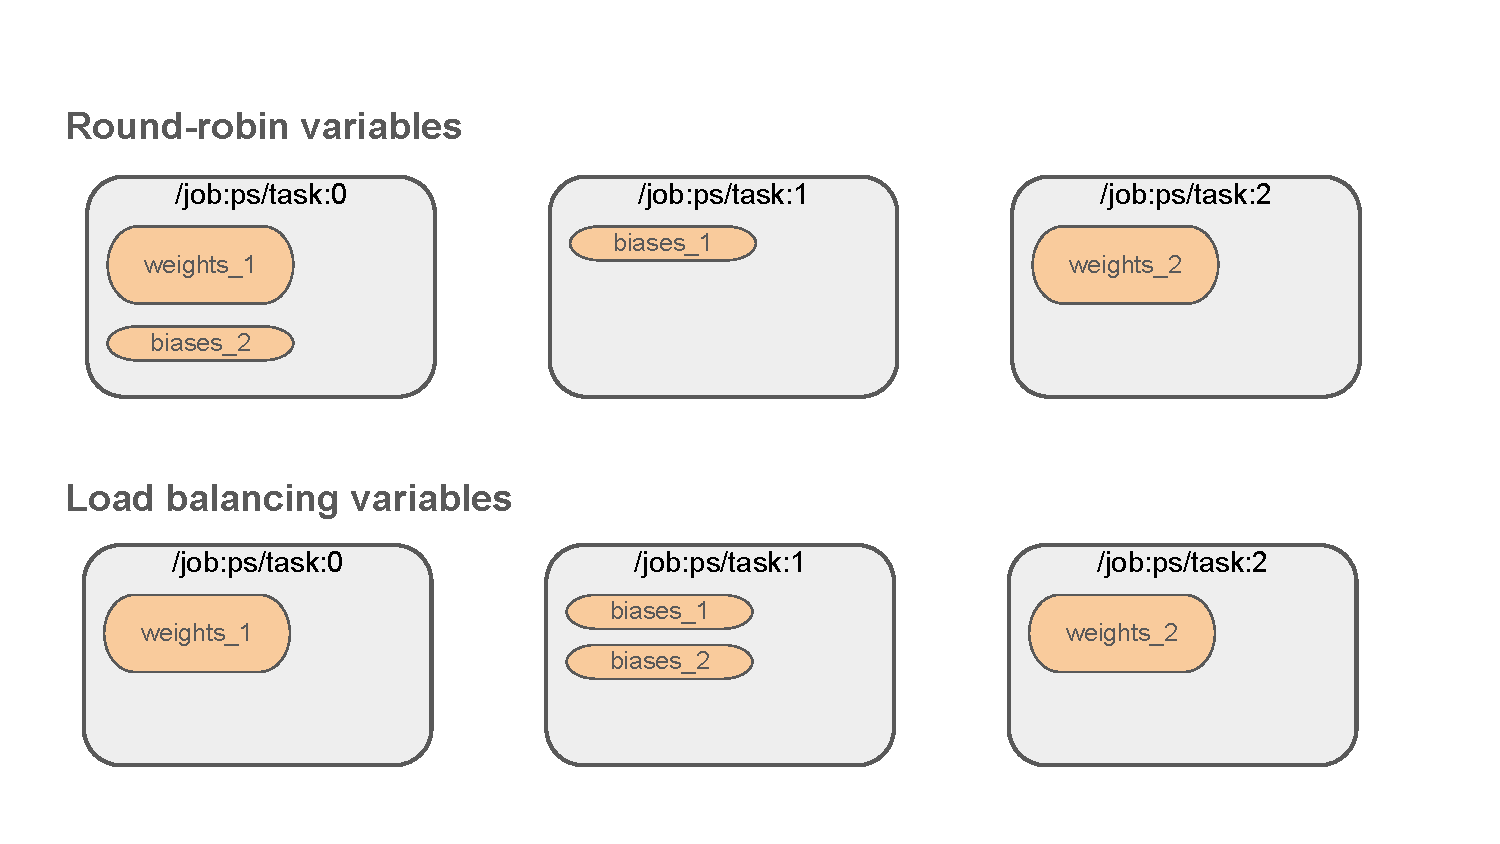
\includegraphics[width=\textwidth,trim={0.5cm 1.2cm 1.5cm 1.7cm},clip]{loadbalancing}
  \vspace{-0.5cm}
  \caption{Round-robin (default) and greedy load balancing variable placement with replica\_device\_setter.} 
  \label{fig:loadbalancing-plot}
\end{figure}
\vspace{-0.3cm}
For this example, Figure \ref{fig:loadbalancing-plot} shows that $\texttt{weights\_1}$ would go to the first Parameter Server, $\texttt{biases\_1}$ would go to the second Parameter Server, $\texttt{weights\_2}$ would be put on the third Parameter Server and $\texttt{biases\_2}$ back on the first Parameter Server.\\
This is obviously not a balance load for these variables, neither in terms of the memory usage nor in terms of the work to be done to update these variables.\\
Moreover, if only two Parameter Servers were used here, we would end up in an even worse case where all the weights would go on the first Parameter Server and all the biases on the second one, giving an even bigger imbalance between these tasks.\\[-0.2cm]

To achieve a more balance load, TensorFlow allows to specify a load balancing strategy in $\texttt{tf.train.replica\_device\_setter}$ as an optional argument.\\
The only one currently available is a simple greedy strategy that does a kind of online bin packing based on the number of bytes of the parameters, giving a more balanced outcome as shown under load balancing variables in Figure \ref{fig:loadbalancing-plot} for our example.
\begin{lstlisting}[label=listing:greedy-loadbalance, language=Python, caption=Greedy load balancing variable placement with \texttt{replica\_device\_setter}.]
greedy =  tf.contrib.training.GreedyLoadBalancingStrategy(...)
with tf.device(tf.train.replica_device_setter(ps_tasks=3, 
                                              ps_strategy=greedy)):
  weights_1 = tf.get_variable('weights_1', [784, 100])
  biases_1 = tf.get_variable('biases_1', [100])
  weights_2 = tf.get_variable('weights_2', [100, 10])
  biases_2 = tf.get_variable('biases_2', [10])
\end{lstlisting}
\newpage

\section{Environments}
In this section, we introduce all the systems which have been used to test and run TensorFlow applications and how to set them up.\\
The version of TensorFlow that we chose is $1.1.0$ in order to compare our results with other benchmarks available online.\\

The code for this section can be found in the $\texttt{environments\_setup}$ folder of our repository.

\subsection{Local workstation}
With local workstation we mean a device, such as a laptop, which usually does not have much compute power.
This can be used to just test whether an application works, even in a distribute setting if it possesses multiple CPUs and/or GPUs.\\

Follow the instructions on the GitHub page to install TensorFlow and create a virtual environment.

\subsection{Piz Daint}
Piz Daint is a hybrid Cray XC40/XC50 supercomputer at CSCS.
The system has Aries routing and communications ASIC, with Dragonfly network topology.\\
At the time of writing, it is the third most powerful supercomputer in the world~\cite{top500} and in the top ten of the most energy-efficient supercomputers~\cite{green500}.\\
Each node that we use in Piz Daint is equipped with an NVIDIA Tesla P100~\cite{p100}.\\

We use the TensorFlow 1.1.0 module available in Piz Daint whenever we run an application.\\
The instructions in the GitHub page show how to create a virtual environment containing all the requirements needed to also run Jupyter notebooks (provided a local workstation has already been set up and its \texttt{pip} requirements are available).

\subsection{AWS EC2}
We also use Amazon EC2 instances~\cite{ec2} to compare the speedup achieved on Piz Daint with the virtual servers available in the cloud of one of the most popular web services.\\
There are many types of virtual servers, also known as compute instances, to choose from~\cite{ec2instances}.
For our comparisons, we make use of P2 instances, intended for general-purpose GPU compute applications.
In particular, we use $p2.xlarge$ (1 GPU per node) and $p2.8xlarge$ (8 GPUs per node) models.\\

\texttt{AWS.md} (in the repository folder) contains additional information on how to create EC2 instances, Amazon S3~\cite{s3} buckets (object storage) and how to transfer data from/to S3.\\
The instructions in the README file illustrate how to set up each instance to run TensorFlow 1.1.0.
To do so, NVIDIA cuDNN~\cite{cudnn} is required.
In our case, we retrieve it from Piz Daint.\\
The only inputs required for the setup of all the machines are their IP addresses, both public and private ones~\footnote{We need the instances' private IP addresses in order to avoid sending each packet through an additional hop, which would considerably reduce performance.}.
Hence, you can simply launch compute instances via the AWS management console and copy their IP addresses, one per line, in $\texttt{aws\_public\_ips.txt}$ and $\texttt{aws\_private\_ips.txt}$ under the repository's root directory, without leaving any empty lines.
\newpage

\section{Distributed TensorFlow}
We now describe how to launch a script written to use distributed TensorFlow (see Section \ref{sec:tf-dist-th}) in each of the environments introduced in the previous section.\\

The code for this section can be found in the $\texttt{distributed\_tensorflow\_launchers}$ folder of our repository.

\subsection{Local workstation}
The setup script for the local workstation runs each task (PS or Worker) on a different terminal window.
By default, Parameter Servers are launched starting at port $2230$, while Workers at $2220$.
The script calls, for each task, $\texttt{run\_dist\_tf\_local.sh}$.\\

This script then runs the (distributed TensorFlow) Python script defined herein, with the flags specified in this file as well, for its corresponding task.

\subsection{Piz Daint}
In the setup script for Piz Daint, we firstly set options for Slurm and load the TensorFlow module.
Then, we define the (distributed TensorFlow) Python script to be executed and its flags.
Finally, we set the number of Parameter Servers and Workers.\\
These values must be consistent with the number of nodes requested for the job.
In particular, if the Parameter Servers run in a (sub)set of the Worker nodes~\footnote{We assume that the number of Workers is always greater than or equal to the number of PSs.} (default behavior), then the number of Workers must not exceed the number of allocated nodes.
On the other hand, if the PSs need to run on different nodes than the Workers, then the total number of tasks must not exceed the number of allocated nodes.
In case the number of allocated nodes is not enough, an error message is returned.\\
Other settings for a distribute run (commented in the setup script) can be tuned.\\
%They are commented in the setup script ($\texttt{setup\_dist\_tf\_daint.sh}$).\\
This script then calls $\texttt{run\_dist\_tf\_daint.sh}$ with the settings declared, which runs the Python script in a distribute environment as described in the next paragraph.\\

$\texttt{run\_dist\_tf\_daint.sh}$ runs the Python script that exported in the setup file.\\
Firstly, the script checks which configuration parameters have been set by the user in the setup file.
The only necessary information needed is the name of the Python script.
The number of Parameter Servers defaults to $1$, while the number of Workers defaults to the number of allocated nodes.
If not set in the setup file, the script also assumes to run one Worker per node and at one Parameter Server.
Note that it is not possible to run multiple Workers on a single node in Piz Daint if you use the GPU partition as multiple TensorFlow tasks cannot share the same device.
As mentioned above, if multiple Parameter Servers are set, the script's default is to run them in a (sub)set of the nodes running a Worker task.
This is possible because Worker's operations run in the GPU, while Parameter Servers run in the CPU.\\
The script then retrieves which nodes have been assigned to the job and creates two comma-separated lists: one indicating Parameter Server hosts and one indicating Worker hosts.
For each node, PSs start at port $2230$, while Workers at port $2220$.\\
After that, for each node, the script determines how many PSs and Workers are to be run in that node, and creates a Bash script to launch Parameter Server and/or Worker processes.
When creating these Bash scripts, if a Parameter Server is to be launched, then it is necessary to hide the GPU to avoid that the PS runs on it; which would result in the Worker running on the CPU.\\
The need of a Bash script is justified by the fact that you can only have a single \texttt{srun} execution per node.
So, we just run each process in background (appending $\texttt{\&}$ at the end of the command) but the last one.

\subsection{AWS EC2}
The setup script for Amazon EC2 instances runs remotely; i.e. from a local workstation, for instance.
It launches one or multiple tasks for each node, according to the number of PSs and Workers entered.
Parameter Servers always run in nodes running Worker tasks as well.
The only inputs to the setup script are the IP addresses of the instances, the path of the private key you use to log into them and the number of PSs and Workers.
In detail, a \texttt{screen} session is started for each task.\\
Parameter Servers' ports start from $2230$ at each node, while Workers' from $2220$.\\
It is necessary that private and public IP addresses correspond to the same EC2 instance in the two IP files. 
That is, the private IP address in line $1$ of the private IP addresses file must be the private address of the instance whose public IP address is in line $1$ in the public IP addresses file.
Private IP addresses are requested in order to reduce the number of hops between two nodes, achieving higher performance.\\

$\texttt{run\_dist\_tf\_aws.sh}$, instead, has to be copied in each EC2 instance, along with the (distributed TensorFlow) Python script.
When called from the setup file, this script firstly hides the GPUs from the Python application if the launched task is a Parameter Server (to the Workers to use them) and then runs the application.

\subsection{Case Study: MNIST}
The \texttt{MNIST} folder of our repository contains an application of the scripts described above for a local workstation and Piz Daint.\\

\texttt{DeepMNIST.ipynb} and \texttt{deepMNIST.py} contain the code of the original deep MNIST tutorial available in TensorFlow's website, which consists of a three-layer neural network (two convolutional layers followed by a fully-connected layer) to classify handwritten digits.\\

We then provide a GPU-enhanced version of this network (\texttt{deepMNIST\_gpu.py}).\\
As described in TensorFlow's High-Performance Models page, one of the best practices to improve performance and increase flexibility of a model is to add the support for the data format.
In fact, most TensorFlow operations used by a CNN support both NHWC and NCHW image data formats.
Image data format refers to the representation of batches of images. 
TensorFlow supports NHWC (TensorFlow default) and NCHW (cuDNN default). 
N refers to the number of images in a batch, H refers to the number of pixels in the vertical dimension, W refers to the number of pixels in the horizontal dimension, and C refers to the channels (e.g. 1 for black and white, 3 for RGB, etc.). 
Although cuDNN can operate on both formats, it is faster to operate in its default format.
So, NCHW should always be used when training with GPUs, while NHWC is sometimes faster on CPUs.
By adding data formats to an application, it is then possible to train using NCHW on GPU, and then do inference with NHWC on CPU.\\
In order to make the existing application support NCHW data format, we introduce some if statements that allow to swap the order of the elements in the \textit{kernel size} and \textit{strides} arrays in the pooling layers.
Moreover, we also use the optional \texttt{data format} argument of the \texttt{tf.nn.conv2d} function to let the specified image data format being used in convolutions.

Finally, we apply the template shown in Listing \ref{listing:tfdist} to train this GPU-enhanced version of MNIST across multiple nodes in \texttt{dist\_deepMNIST\_gpu.py}.
Here, only Worker 0 evaluates test accuracy, while each Worker evaluates their train accuracy.
To launch this application, we used the setup and run\_dist\_tf scripts presented in this section.
\newpage

\section{Benchmarking Distributed Training}
We now present the scalability results relative to training InceptionV3~\cite{inception3}, a deep neural network by Google, on GPU-enabled nodes in Piz Daint and in Amazon EC2.\\
To do so, we use Google's script~\cite{cnn_benchmarks}, which provides optimized implementations for multiple networks.
The dataset used for training is ImageNet~\cite{imagenet}, one of the most common datasets used for classification in Computer Vision.\\

The code for this section can be found in the \texttt{google-benchmarks} folder of our repository.

\subsection{Methodology}
Google's script allows to set different parameters, such as the batch size, the number of warmup steps, the number of steps to be averaged, whether to use NVIDIA NCCL all-reduce primitives and the data layout format (NCHW or NHWC).\\

The main output of this script is the average number of images per second that have been trained in the system.
In order to find a good ratio between the number of Workers and the number of Parameter Servers, we try, for each configuration of number of Workers and number of nodes, several values for the number of PSs ranging from $1$ to the number of Workers.
For each configuration, we then report the results achieving the largest number of images trained per second.
In order to produce results that are as repeatable as possible, each test was run 5 times and then the times were averaged together, analogously to what Google did. 
GPUs are run in their default state on all the platforms.\\
For each test, 10 warmup steps are done and then the next 100 steps are averaged.\\

We ran our benchmarks using both real and synthetic data~\footnote{By synthetic data we mean fake data that has almost the same properties as the real one.}, so that we can evaluate both the compute and the input pipelines.

\subsection{Systems}
We run benchmarks on Piz Daint, as well as on \textit{p2.xlarge} and \textit{p2.8xlarge} Amazon EC2 instances.
Whenever possible, we compare our results with the ones published by Google~\cite{google_benchmarks}, obtained with \textit{NVIDIA DGX-1} and Amazon \textit{p2.8xlarge} systems.\\
Piz Daint and NVIDIA DGX-1 both have NVIDIA Tesla P100 GPUs, even though the former only has one GPU per node, while the latter has 8 GPUs per node.
Amazon \textit{p2.xlarge} and \textit{p2.8xlarge} EC2 instances, instead, are equipped with NVIDIA Tesla K80 GPUs. 
\textit{p2.xlarge} instances have one GPU per node, while \textit{p2.8xlarge} instances have eight GPUs per node (four K80).

\subsection{Results}
For all of the reported results, the following settings are used: 
\begin{itemize}
	\item \textbf{Model:} InceptionV3
	\item \textbf{Batch size per GPU:} 64
    \item \textbf{Data Format:} NCHW
    \item \textbf{Local Parameter Device:} CPU
	\item \textbf{Optimizer:} sgd
    \item \textbf{Piz Daint OS:} Suse 12/CLE 6.0.UP02
    \item \textbf{AWS OS:} Ubuntu 16.04 LTS
    \item \textbf{CUDA/cuDNN:} 8.0/5.1
    \item \textbf{TensorFlow:} 1.1.0
    \item \textbf{Piz Daint Parallel File System:} Lustre
    \item \textbf{AWS Disk:} Local SSD
    \item \textbf{DataSet:} ImageNet
	\item \textbf{Test Date:} August 2017
\end{itemize}
Moreover, nodes running Workers also run Parameter Servers as this leads to higher performance.

\subsubsection{Training with NVIDIA Tesla P100}
Google provides results only for a single NVIDIA DGX-1, hence allowing comparisons up to 8 GPUs.
Results are shown in Figure \ref{fig:dgx-daint} for synthetic data (no I/O).
\begin{figure}[t]
  \centering
  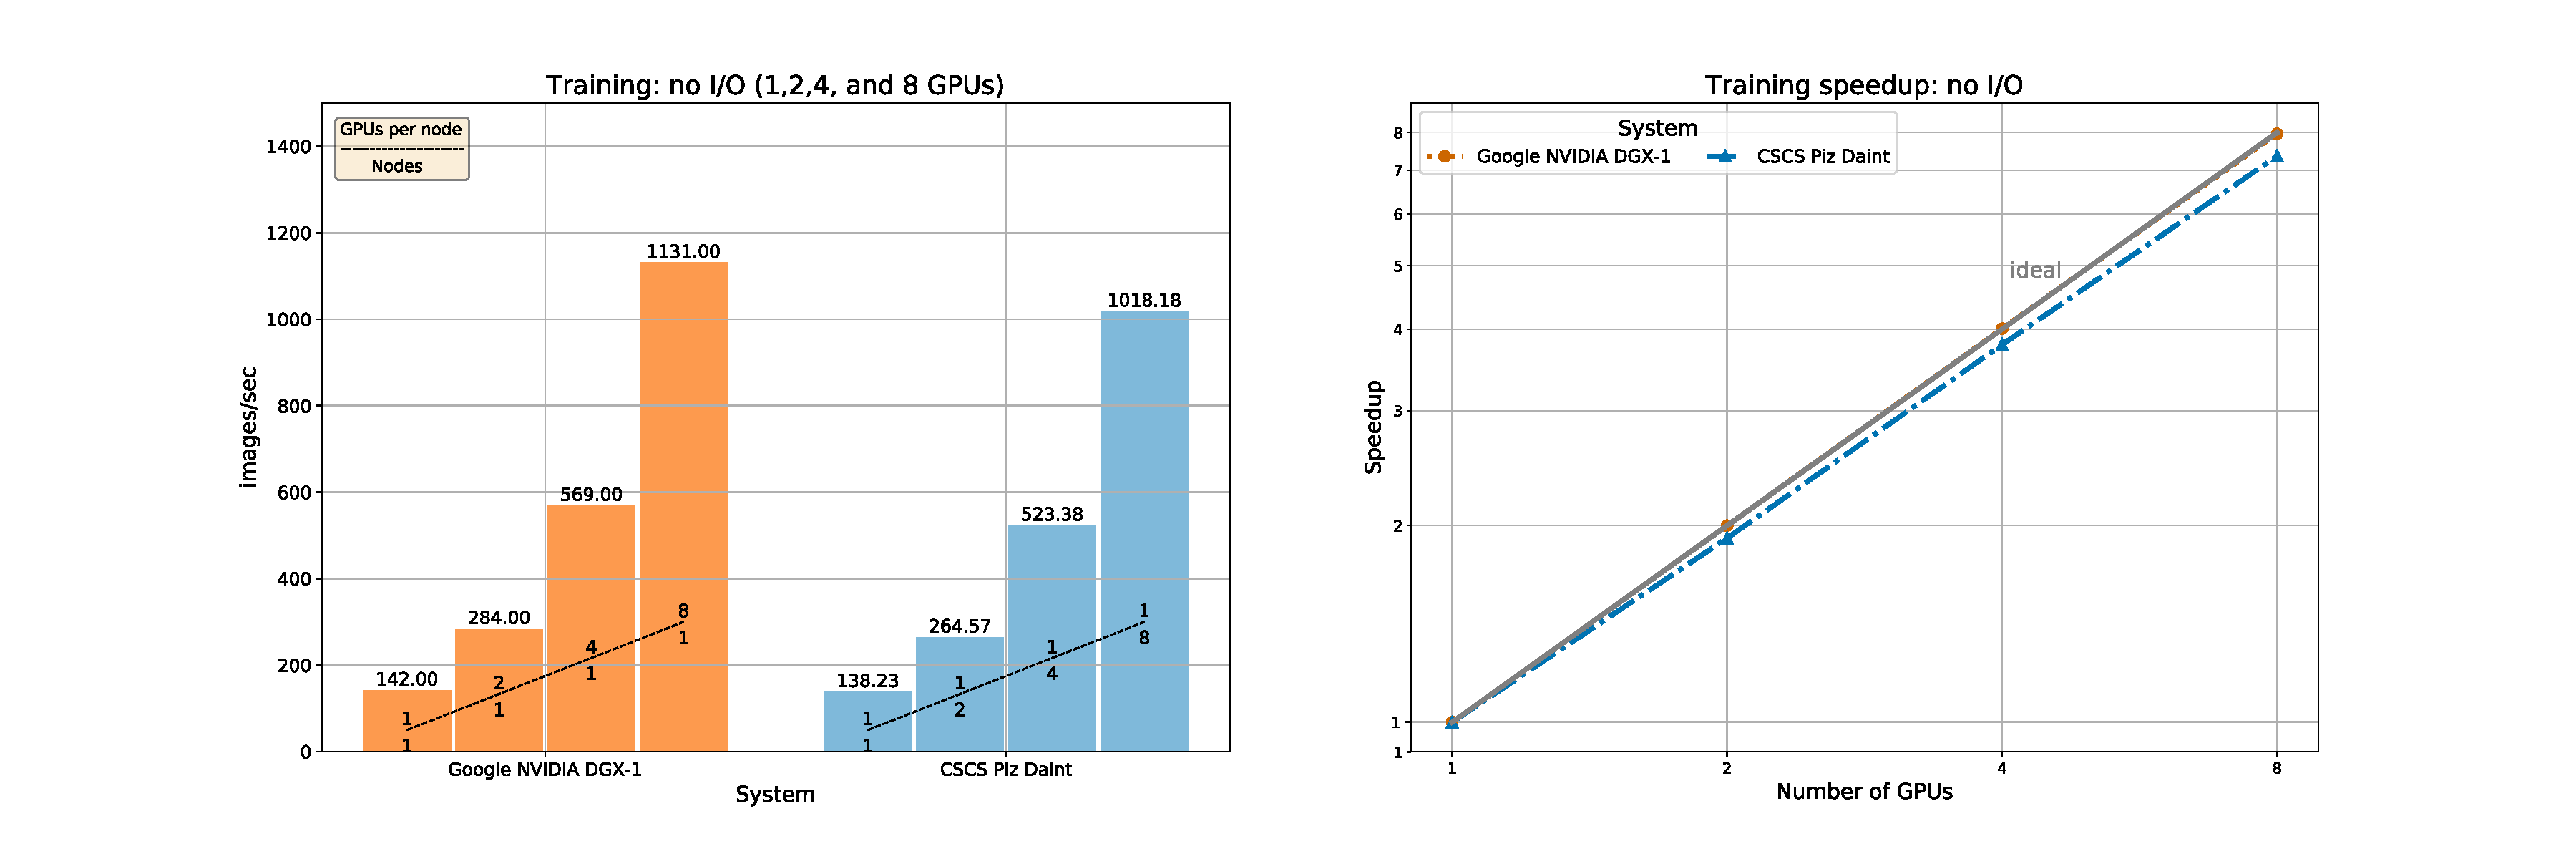
\includegraphics[width=\textwidth,trim={4cm 1.2cm 4.5cm 1.7cm},clip]{google-daint-synthetic.pdf}
  \vspace{-0.85cm}
  \caption{Training with NVIDIA Tesla P100 on synthetic data up to 8 GPUs.} 
  \label{fig:dgx-daint}
\end{figure}
Here, we can see that the peak performance of Piz Daint is close to the one achieved by an NVIDIA DGX-1, even though multiple nodes are used in Piz Daint.
Specifically, with eight GPUs, while Google reports a speedup efficiency of $99.56\%$, we report a speedup efficiency of $92.07\%$ on Piz Daint.

\vspace{-0.3cm}
\subsubsection{Training with NVIDIA Tesla K80}
\vspace{-0.2cm}
Figure \ref{fig:aws-google-cscs} shows how Amazon EC2 \textit{p2.xlarge} and \textit{p2.8xlarge} compute instances scale out up to 8 GPUs.
\begin{figure}[H]
  \centering
  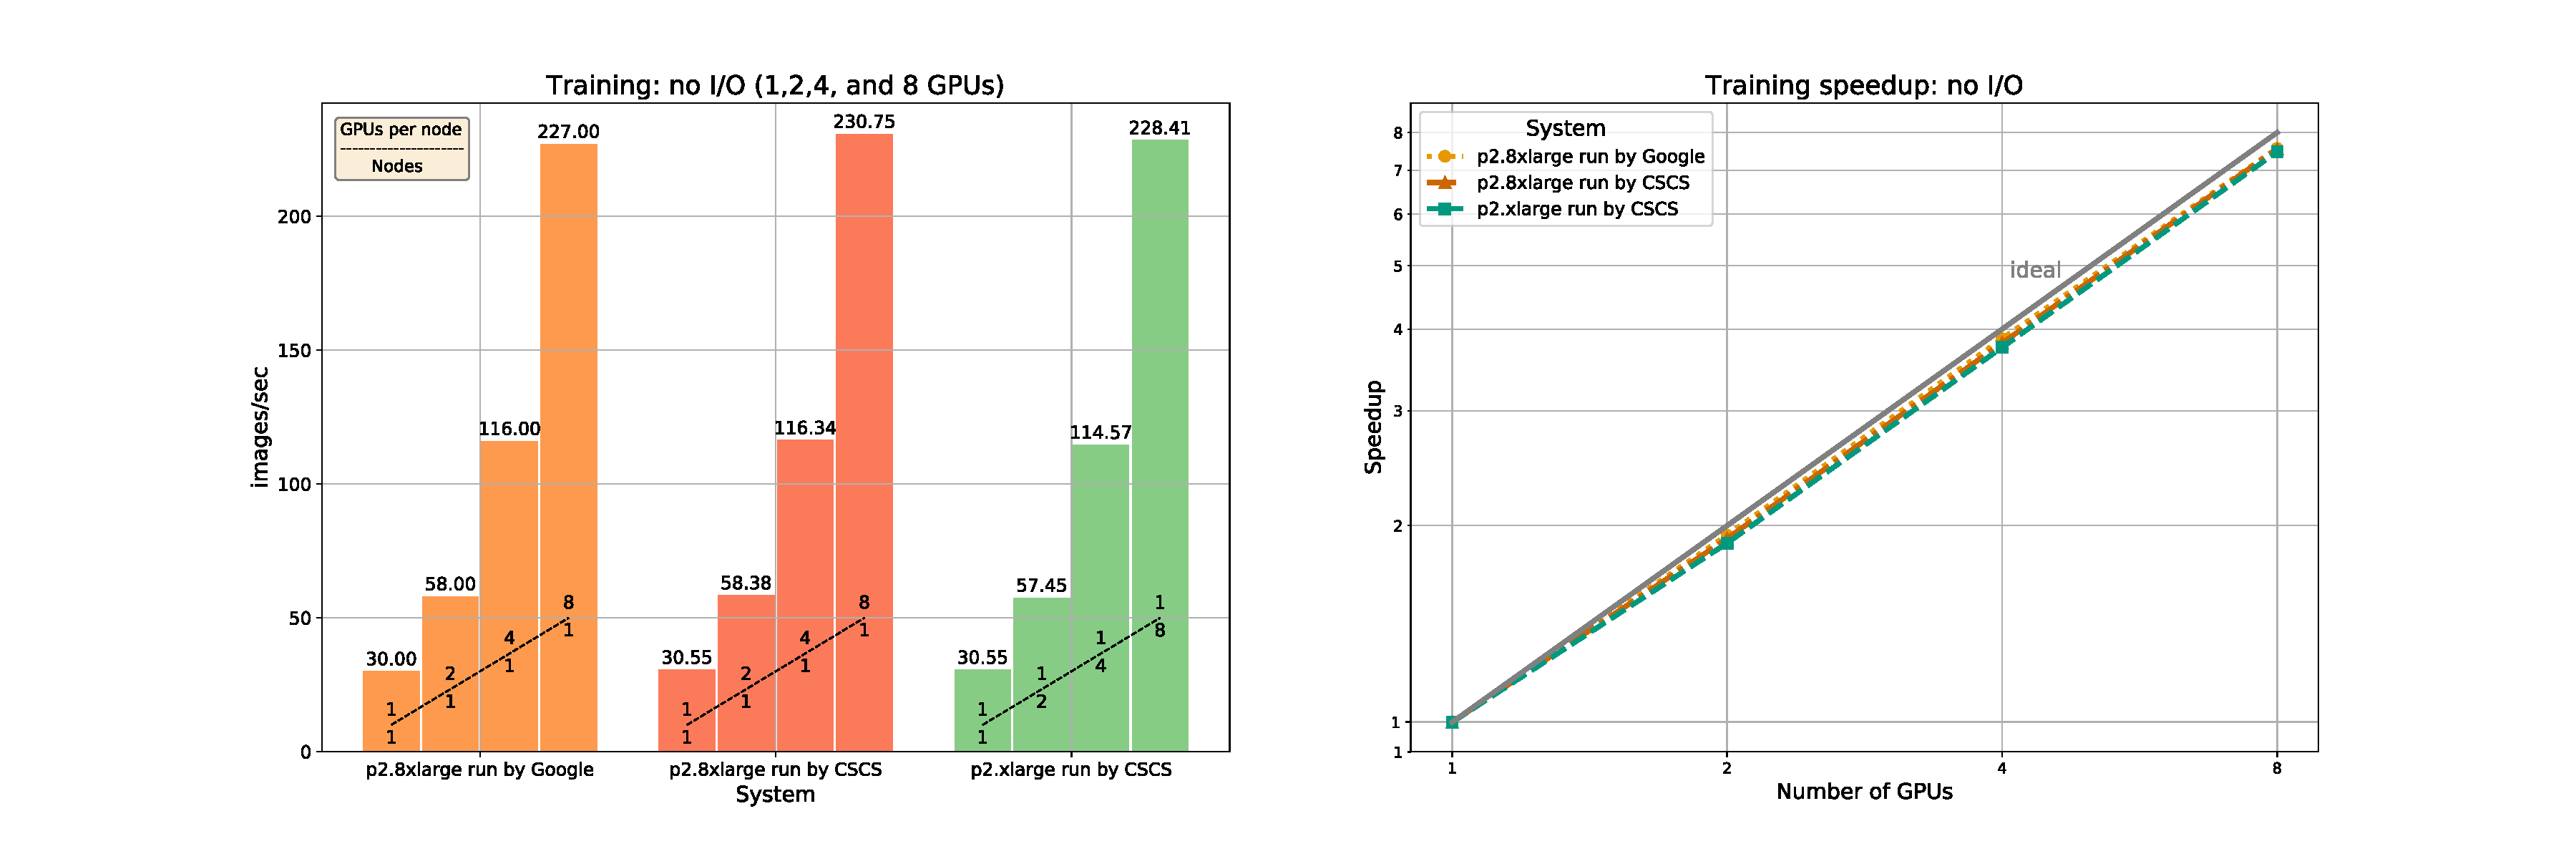
\includegraphics[width=\textwidth,trim={4cm 1.2cm 4.5cm 1.7cm},clip]{google-our-aws-synthetic.pdf}
  \vspace{-0.85cm}
  \caption{Training with NVIDIA Tesla K80 on synthetic data up to 8 GPUs.} 
  \label{fig:aws-google-cscs}
\end{figure}
\vspace{-0.2cm}
Google provides results that achieve a scalability efficiency of $94.58\%$ with 8 GPUs on a \textit{p2.8xlarge}, and, similarly, our measurements show an efficiency of $94.44\%$ on the same machine.\\
We also ran tests on \textit{p2.xlarge} instances, showing that comparable performance ($93.45\%$ scalability efficiency) can be obtained with eight nodes (eight GPUs).\\
Hence, we can infer that the application is compute bounded when up to eight GPUs are used because we achieve the same performance with eight nodes as with a single node having eight GPUs regardless of the underlying network (Piz Daint or AWS).\\

Figure \ref{fig:dist-aws-google-cscs}, instead, shows how the number of images trained per second in these systems scales when up to 64 GPUs are used.
\begin{figure}[t]
  \centering
  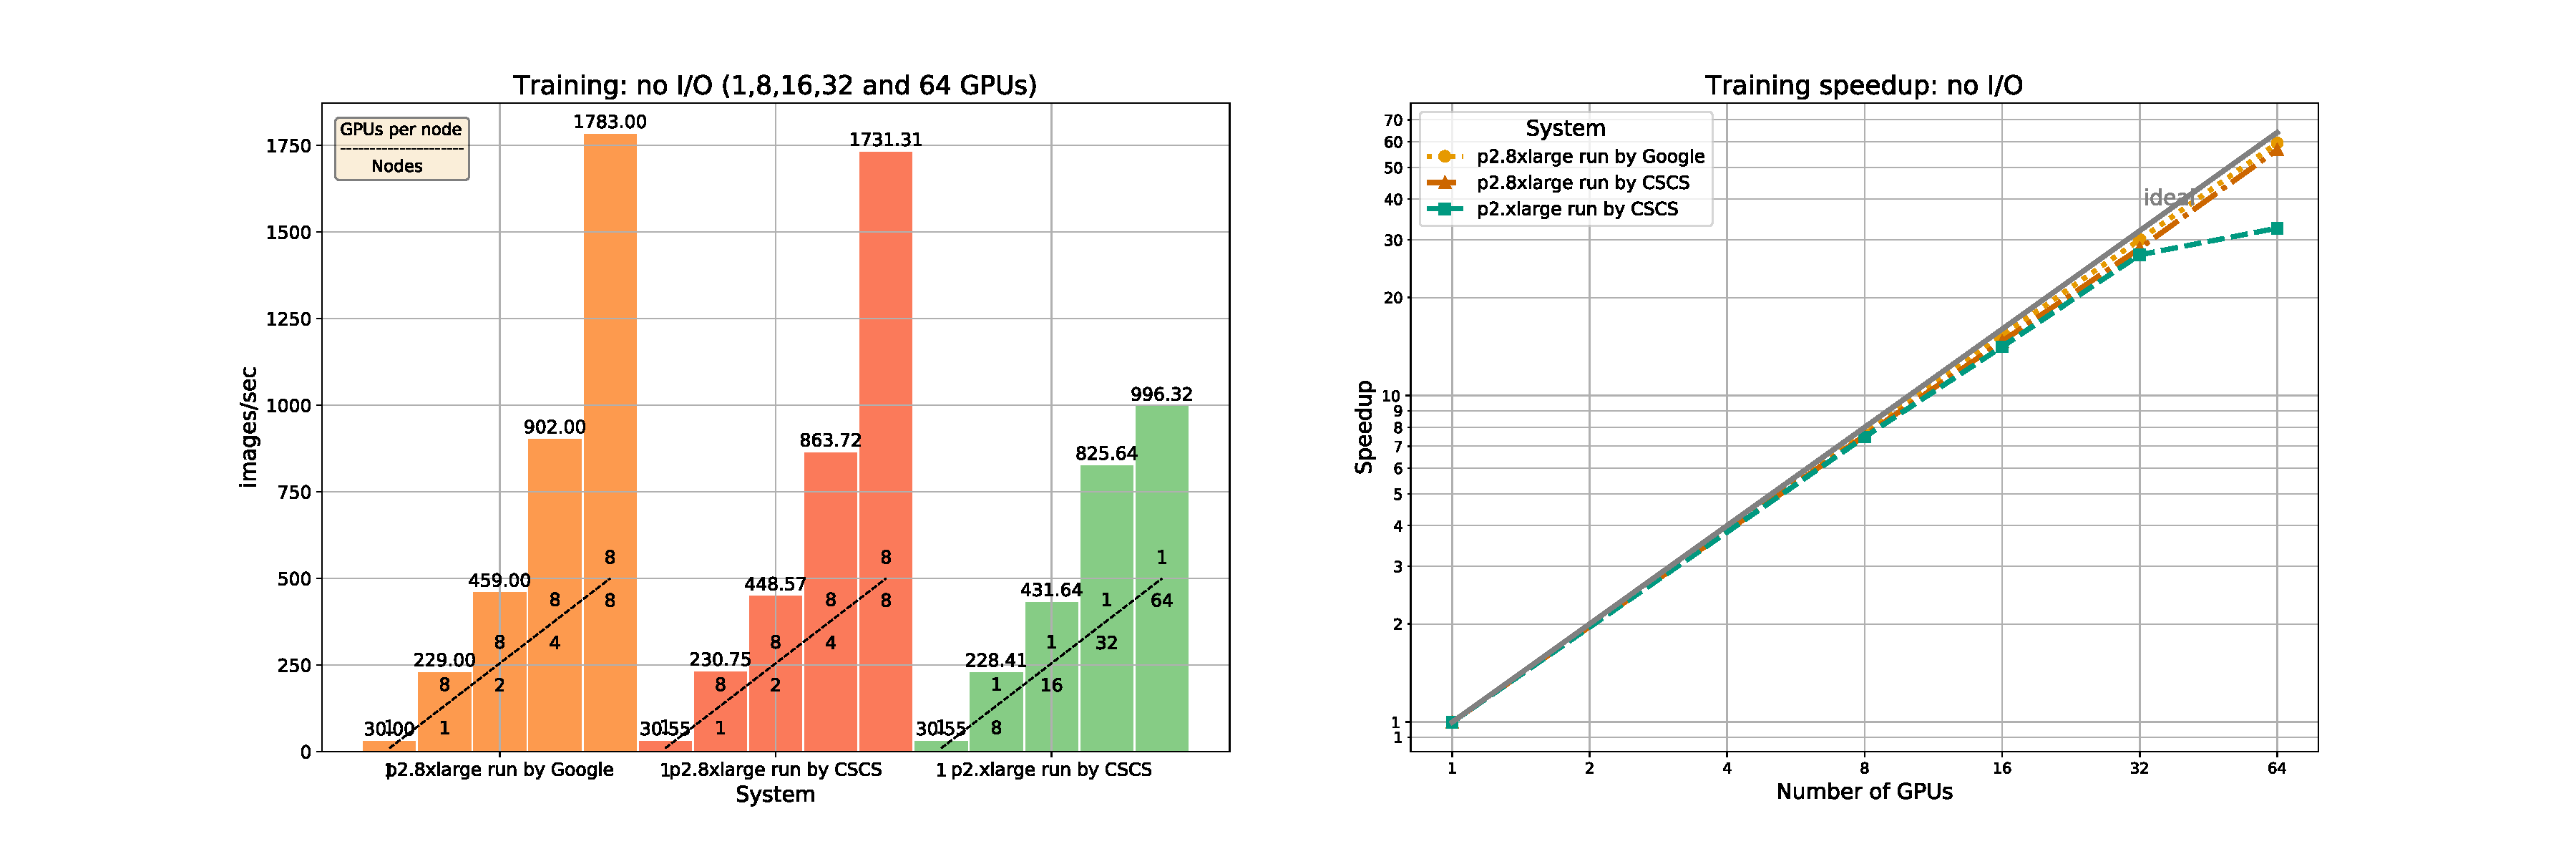
\includegraphics[width=\textwidth,trim={4cm 1.2cm 4.5cm 1.7cm},clip]{google-our-dist-aws-synthetic.pdf}
  \vspace{-0.85cm}
  \caption{Training with NVIDIA Tesla K80 on synthetic data up to 64 GPUs.} 
  \label{fig:dist-aws-google-cscs}
\end{figure}
% \vspace{-0.5cm}
It is interesting to note that up to 16 GPUs, \textit{p2.xlarge} and \textit{p2.8xlarge} systems have close performance: We report $88.31\%$ for the former and $91.77\%$ for the latter.\\
Moreover, even though 32 nodes are required for a \textit{p2.xlarge} system to use 32 GPUs, it still achieves a scalability efficiency greater than $80\%$.
Specifically, we report $88.35\%$ efficiency for a four-node \textit{p2.8xlarge} system and $84.45\%$ efficiency for a thirty-two-node \textit{p2.xlarge} system.\\
However, once a cluster of sixty-four \textit{p2.xlarge} nodes is employed, the scalability efficiency stops at $50.96\%$, while a cluster of eight \textit{p2.8xlarge} still exhibits $88.55\%$ efficiency from our measurements and $92.86\%$ from Google's ones.
This is probably due to the fact that the network capacity is not sufficient anymore for the amount of traffic generated by all the nodes in the \textit{p2.xlarge} cluster.

\subsubsection{Distributed training on Piz Daint}
Figure \ref{fig:daint} shows how the average number of images trained per second varies as the number of nodes (GPUs) increases both when using fake data and when reading data from the Parallel File System on Piz Daint.
Each of these values represents the peak performance achieved with the corresponding number of GPUs, obtained by setting the parameters listed in Table \ref{tab:peak-perf-daint}.
Here, we can see that Piz Daint's scalability efficiency drastically drops when 128 nodes are used.
We think this is due to having reached the inter-node network capacity because of the largely increased amount of data sent between Workers and Parameter Servers.
\begin{figure}[H]
  \centering
  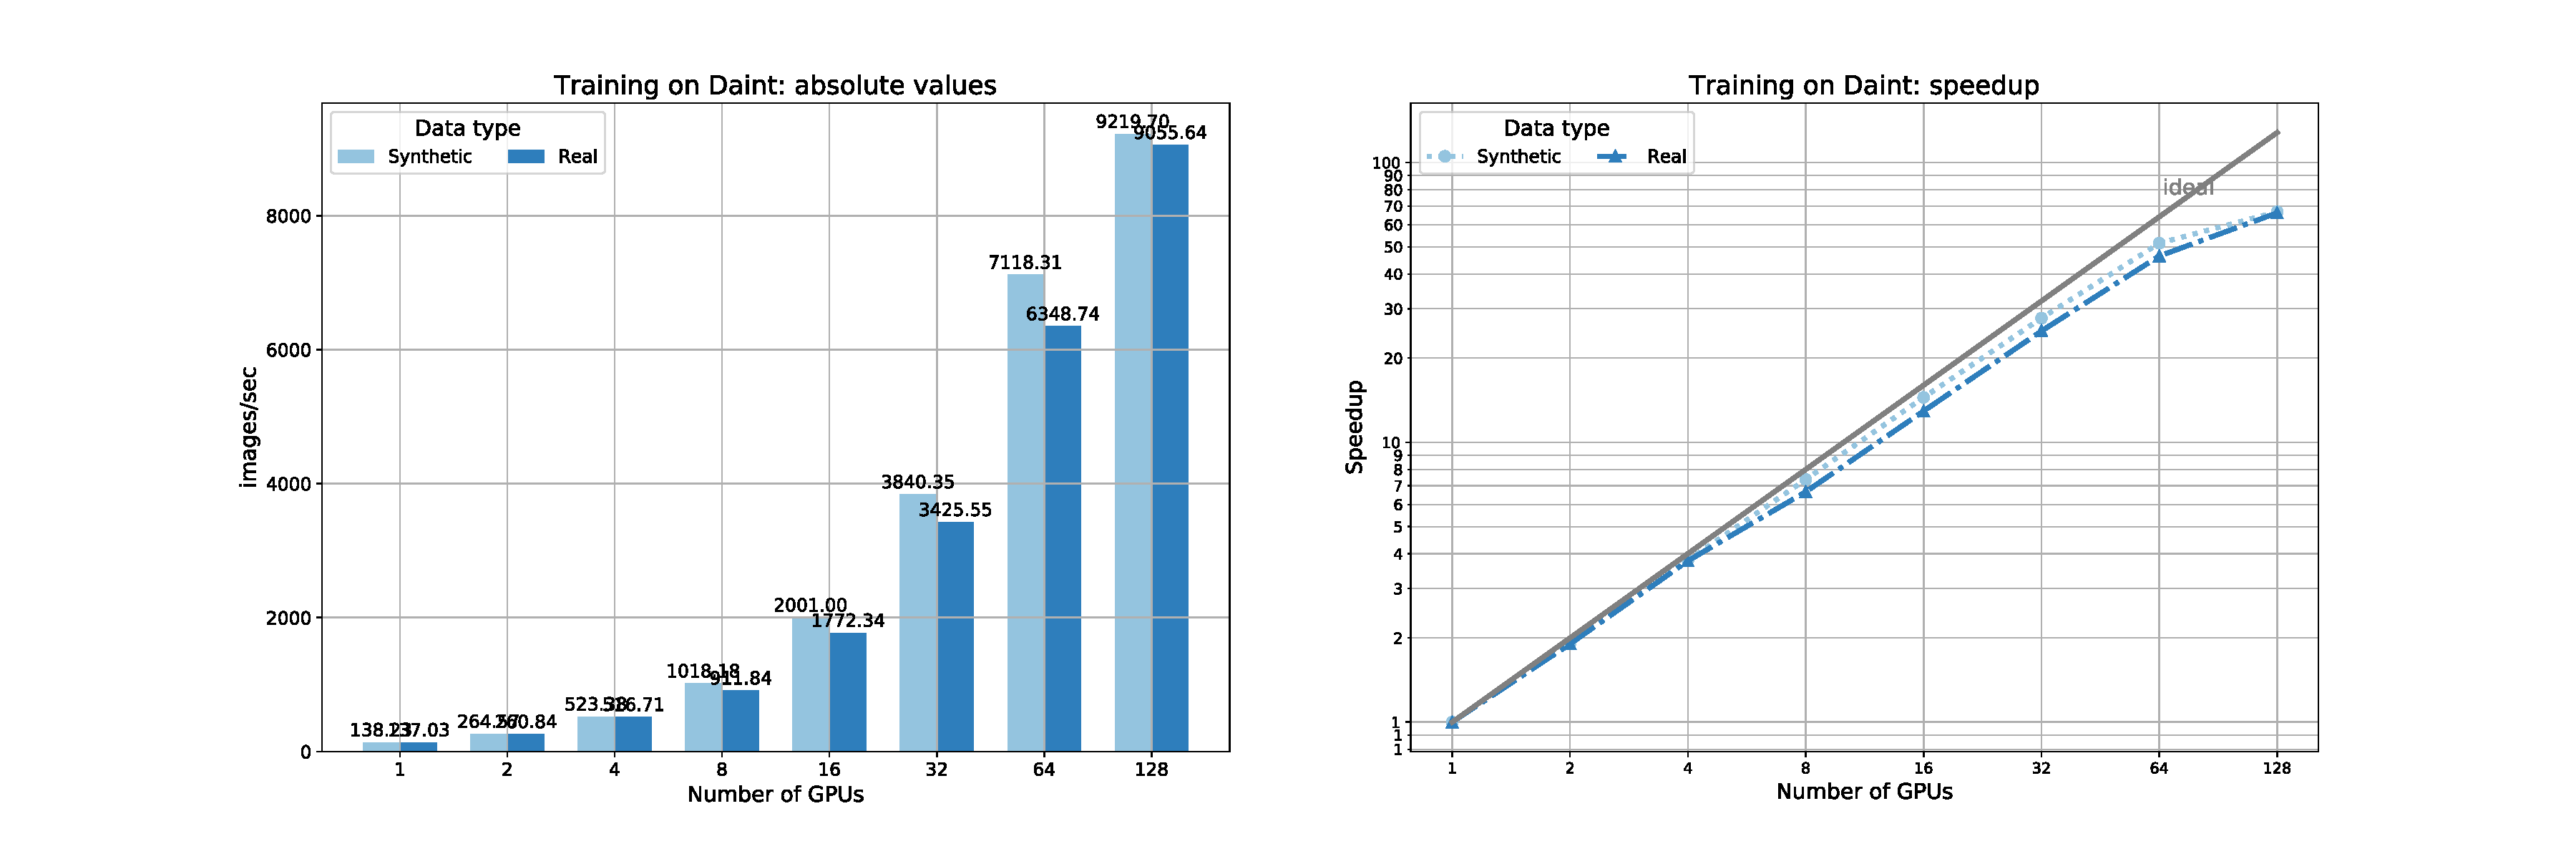
\includegraphics[width=\textwidth,trim={4cm 1.2cm 4.5cm 1.7cm},clip]{daint-synthetic-real.pdf}
  \vspace{-0.85cm}
  \caption{Training on Piz Daint with synthetic and real data up to 128 GPUs.} 
  \label{fig:daint}
\end{figure}
% \vspace{-0.5cm}
\begin{table}[H]
 \centering
 \begin{tabular}{||l | l | l | l | r||} 
 \hline
 \textbf{Num PSs} & \textbf{Num GPUs} & \textbf{Variable Update} & \textbf{Real Data} & \textbf{Img/s}\\ [0.5ex] 
 \hline\hline
 1 & 1 & parameter\_server & FALSE & 138.23\\\hline
 1 & 1 & parameter\_server & TRUE & 137.03\\\hline
 1 & 2 & parameter\_server & FALSE & 264.57\\\hline
 1 & 2 & distributed\_replicated & TRUE & 260.84\\\hline
 3 & 4 & distributed\_replicated & FALSE & 523.38\\\hline
 3 & 4 & distributed\_replicated & TRUE & 516.71\\\hline
 2 & 8 & parameter\_server & FALSE & 1018.18\\\hline
 2 & 8 & parameter\_server & TRUE & 911.84\\\hline
 4 & 16 & parameter\_server & FALSE & 2001.00\\\hline
 4 & 16 & parameter\_server & TRUE & 1772.34\\\hline
 12 & 32 & parameter\_server & FALSE & 3840.35\\\hline
 12 & 32 & parameter\_server & TRUE & 3425.55\\\hline
 40 & 64 & parameter\_server & FALSE & 7118.31\\\hline
 40 & 64 & parameter\_server & TRUE & 6348.74\\\hline
 116 & 128 & parameter\_server & FALSE & 9219.70\\\hline
 116 & 128 & parameter\_server & TRUE & 9055.64\\\hline
\end{tabular}
\caption{Parameters achieving peak performance on Piz Daint.}
\label{tab:peak-perf-daint}
\end{table}

\subsubsection{Distributed training on Amazon p2.xlarge}
Figure \ref{fig:p2} displays the trend of average number of images trained per second as the number of nodes (GPUs) increases both when using fake data and when reading data from the local SSD at each node in a cluster of \textit{p2.xlarge} machines.
The parameters resulting in the peak performance for each different number of GPUs are listed in Table \ref{tab:peak-perf-p2}.
In this plot, we can see that \textit{p2.xlarge}'s scalability efficiency diminishes only when 64 nodes are benchmarked.
This system has single-GPU nodes like Piz Daint but it stops scaling out efficiently for a smaller number of nodes.
The main difference amongst them is their inter-node network (Piz Daint's being faster), providing additional support to our belief of inter-node network bottleneck for Piz Daint and \textit{p2.xlarge} systems.
\begin{figure}[H]
  \centering
  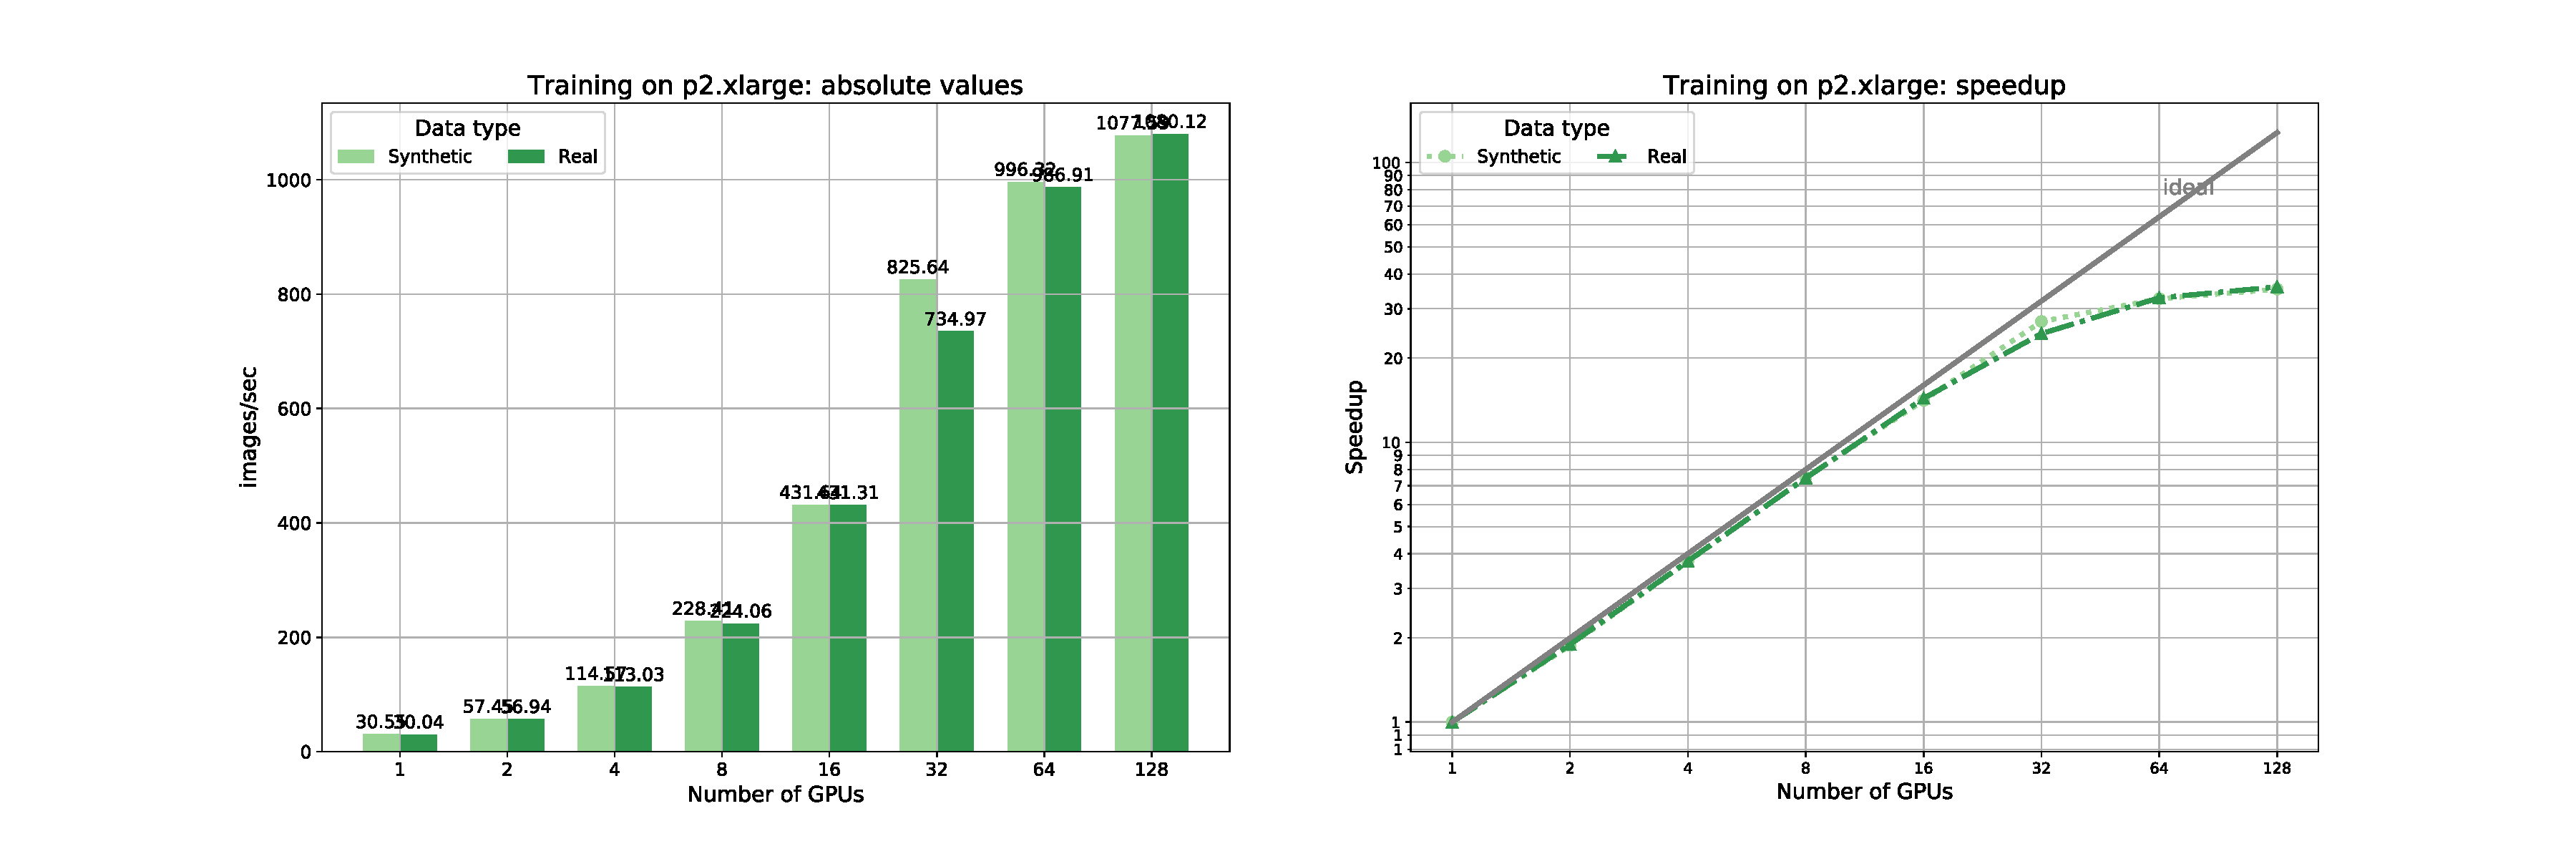
\includegraphics[width=\textwidth,trim={4cm 1.2cm 4.5cm 1.7cm},clip]{p2-synthetic-real.pdf}
  \vspace{-0.85cm}
  \caption{Training on \textit{p2.xlarge} with synthetic and real data up to 128 GPUs.}
  \label{fig:p2}
\end{figure}
% \vspace{-0.5cm}
\begin{table}[H]
 \centering
 \begin{tabular}{||l | l | l | l | r||} 
 \hline
\textbf{Num PSs} & \textbf{Num GPUs} & \textbf{Variable Update} & \textbf{Real Data} & \textbf{Img/s}\\ [0.5ex] 
\hline\hline
 1 & 1 & parameter\_server & FALSE & 30.55\\\hline
 1 & 1 & parameter\_server & TRUE & 30.04\\\hline
 2 & 2 & distributed\_replicated & FALSE & 57.45\\\hline
 2 & 2 & distributed\_replicated & TRUE & 56.93\\\hline
 4 & 4 & distributed\_replicated & FALSE & 114.57\\\hline
 4 & 4 & distributed\_replicated & TRUE & 113.03\\\hline
 8 & 8 & distributed\_replicated & FALSE & 228.41\\\hline
 8 & 8 & distributed\_replicated & TRUE & 224.06\\\hline
 12 & 16 & distributed\_replicated & FALSE & 431.64\\\hline
 12 & 16 & distributed\_replicated & TRUE & 431.31\\\hline
 32 & 32 & parameter\_server & FALSE & 825.64\\\hline
 32 & 32 & parameter\_server & TRUE & 734.97\\\hline
 64 & 64 & parameter\_server & FALSE & 996.32\\\hline
 64 & 64 & parameter\_server & TRUE & 986.91\\\hline
 128 & 128 & parameter\_server & FALSE & 1077.59\\\hline
 128 & 128 & parameter\_server & TRUE & 1080.12\\\hline
\end{tabular}
\caption{Parameters achieving peak performance on \textit{p2.xlarge} systems.}
\label{tab:peak-perf-p2}
\end{table}

\subsubsection{Distributed training on Amazon p2.8xlarge}
\vspace{-0.2cm}
Figure \ref{fig:p28} presents the average number of images trained per second as a function of the number of GPUs both when using fake data and when reading data from local the SSD at each node in a \textit{p2.8xlarge} cluster.
The parameters giving the highest performance for the different numbers of GPUs are enlisted in Table \ref{tab:peak-perf-p28}.
This plot does not show any evident reduction in scalability as the number of GPUs is increased.
In such system, Workers aggregate their updates before sending them to the PSs. 
Hence, the traffic generated when 128 GPUs are used here is comparable to the one generated by a system of sixteen single-GPU nodes.
\vspace{-0.2cm}
\begin{figure}[H]
  \centering
  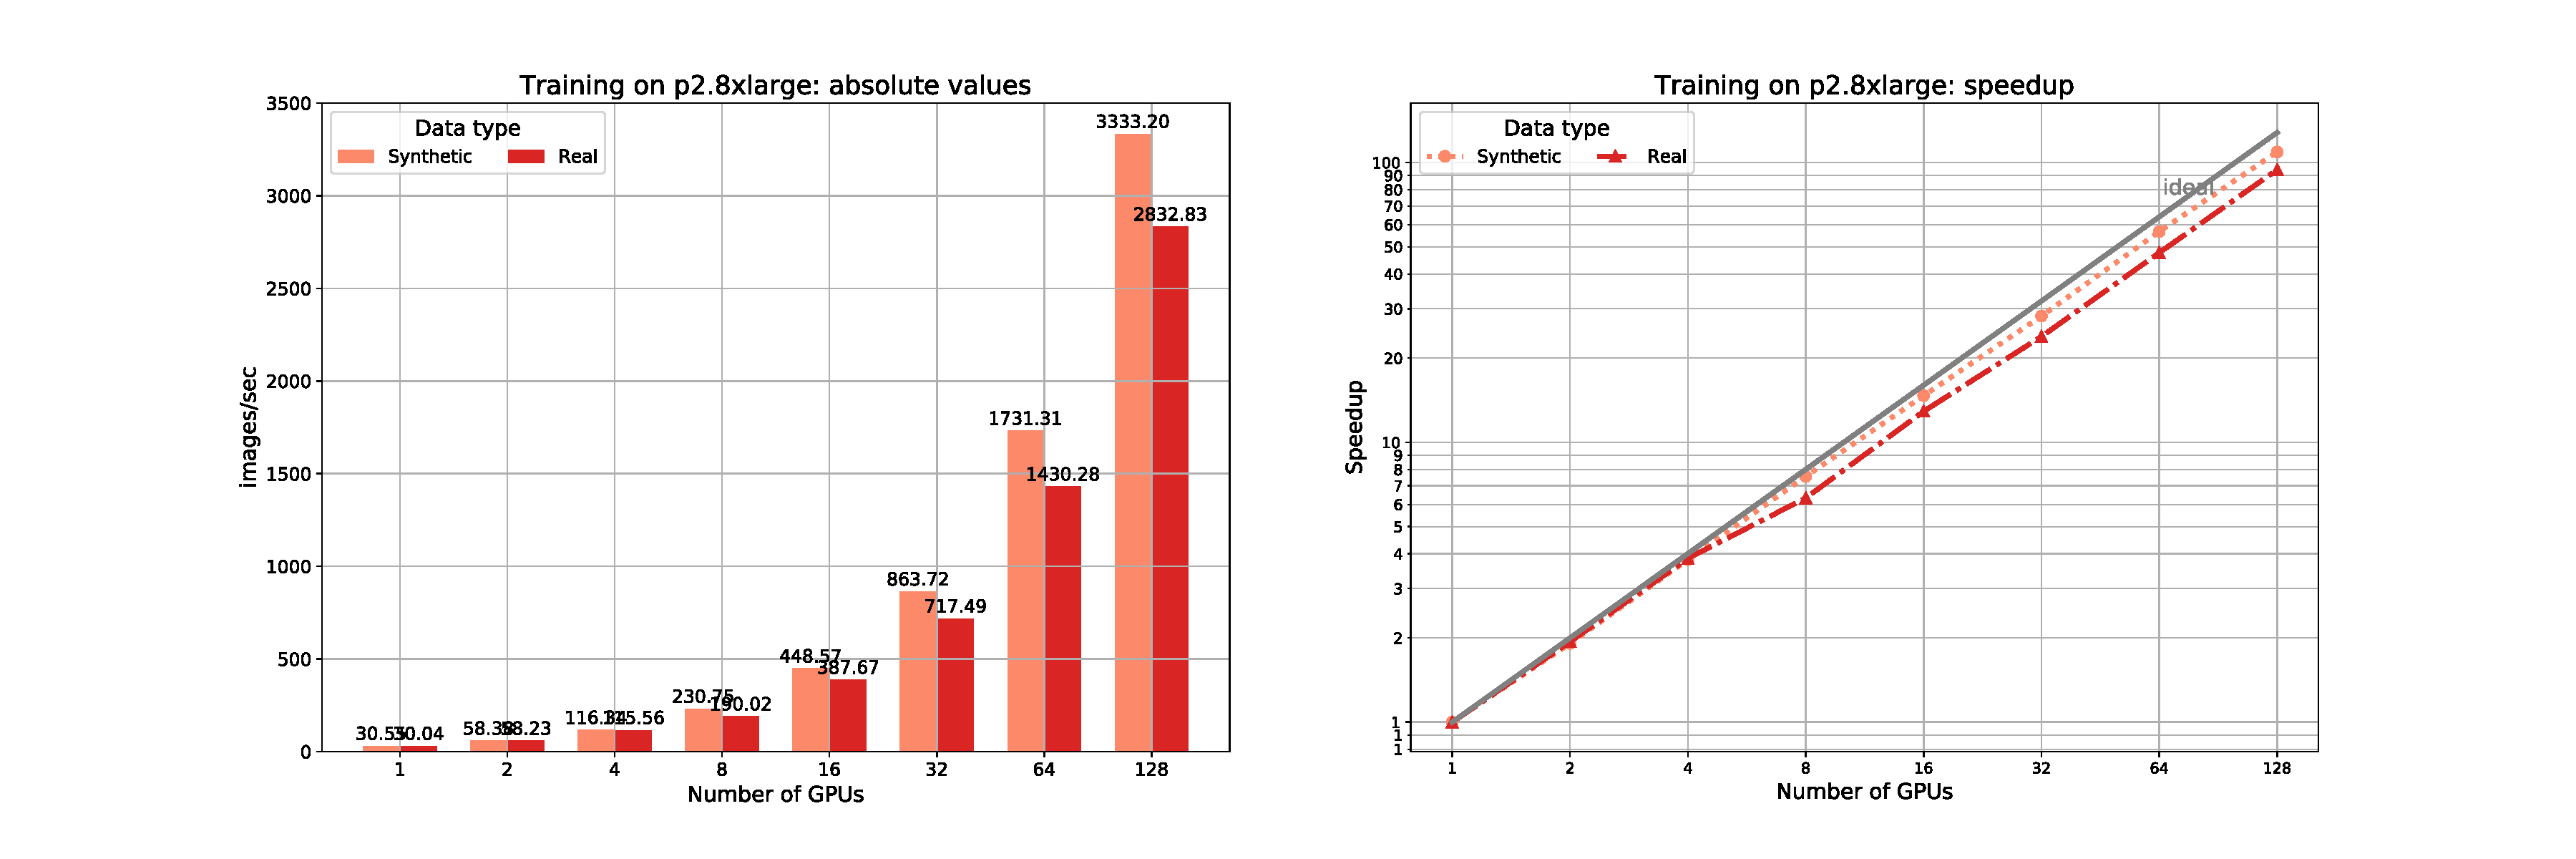
\includegraphics[width=\textwidth,trim={4cm 1.2cm 4.5cm 1.7cm},clip]{p28-synthetic-real.pdf}
  \vspace{-0.85cm}
  \caption{Training on \textit{p2.8xlarge} with synthetic and real data up to 128 GPUs.}
  \label{fig:p28}
\end{figure}
\vspace{-0.55cm}
\begin{table}[H]
 \centering
 \begin{tabular}{||l | l | l | l | r||} 
 \hline
 \textbf{Num PSs} & \textbf{Num GPUs} & \textbf{Variable Update} & \textbf{Real Data} & \textbf{Img/s}\\ [0.5ex]  
 \hline\hline
 1 & 1 & parameter\_server & FALSE & 30.55\\\hline
 1 & 1 & parameter\_server & TRUE & 30.04\\\hline
 1 & 2 & distributed\_replicated & FALSE & 58.38\\\hline
 1 & 2 & distributed\_replicated & TRUE & 58.23\\\hline
 1 & 4 & distributed\_replicated & FALSE & 116.34\\\hline
 1 & 4 & distributed\_replicated & TRUE & 115.56\\\hline
 1 & 8 & distributed\_replicated & FALSE & 230.75\\\hline
 1 & 8 & distributed\_replicated & TRUE & 190.02\\\hline
 1 & 16 & distributed\_replicated & FALSE & 448.57\\\hline
 1 & 16 & distributed\_replicated & TRUE & 387.67\\\hline
 3 & 32 & distributed\_replicated & FALSE & 863.72\\\hline
 3 & 32 & distributed\_replicated & TRUE & 717.49\\\hline
 8 & 64 & distributed\_replicated & FALSE & 1731.31\\\hline
 8 & 64 & distributed\_replicated & TRUE & 1430.28\\\hline
 16 & 128 & distributed\_replicated & FALSE & 3333.20\\\hline
 16 & 128 & distributed\_replicated & TRUE & 2832.83\\\hline
\end{tabular}
\caption{Parameters achieving peak performance on \textit{p2.8xlarge} systems.}
\label{tab:peak-perf-p28}
\end{table}

\subsubsection{I/O overhead}
Finally, Figure \ref{fig:io} plots the relative overhead (in percentage) due to I/O access.
That is, for each setting, we obtain the relative I/O in percentage as:
$$I/O~overhead~_{System}^{N\_GPUs} = \dfrac{Img/s\_Synthetic_{System}^{N\_GPUs} - Img/s\_Real_{System}^{N\_GPUs}}{Img/s\_Synthetic_{System}^{N\_GPUs}} \times 100.$$

The first thing we observe from this plot is that when 8 GPUs per node are used in a \textit{p2.8xlarge} cluster, where each node loads data from a local SSD, a constant I/O overhead of around $17\%$ is present (due to PCIe traffic).\\

Looking at \textit{p2.xlarge} clusters, instead, we see that I/O access does not add any overhead, apart when thirty-two nodes are used.
However, this still comes at the expenses of replicating the data at each node.\\

Focusing on Piz Daint at last, we see that around $11\%$ of I/O overhead is present when eight to sixty-four nodes are used.\\
On the other hand, this is not shown when less nodes are employed.
The reason might be due to caching mechanisms in the system.\\
The I/O overhead drops down once more for one hundred and twenty-eight nodes.
In this case, the reason of this reduction may be found in the predominance of the inter-node network bottleneck, which makes the impact of I/O access negligible.\\

TensorFlow communication patterns should be profiled to verify all our intuitions.

\begin{figure}[t]
  \centering
  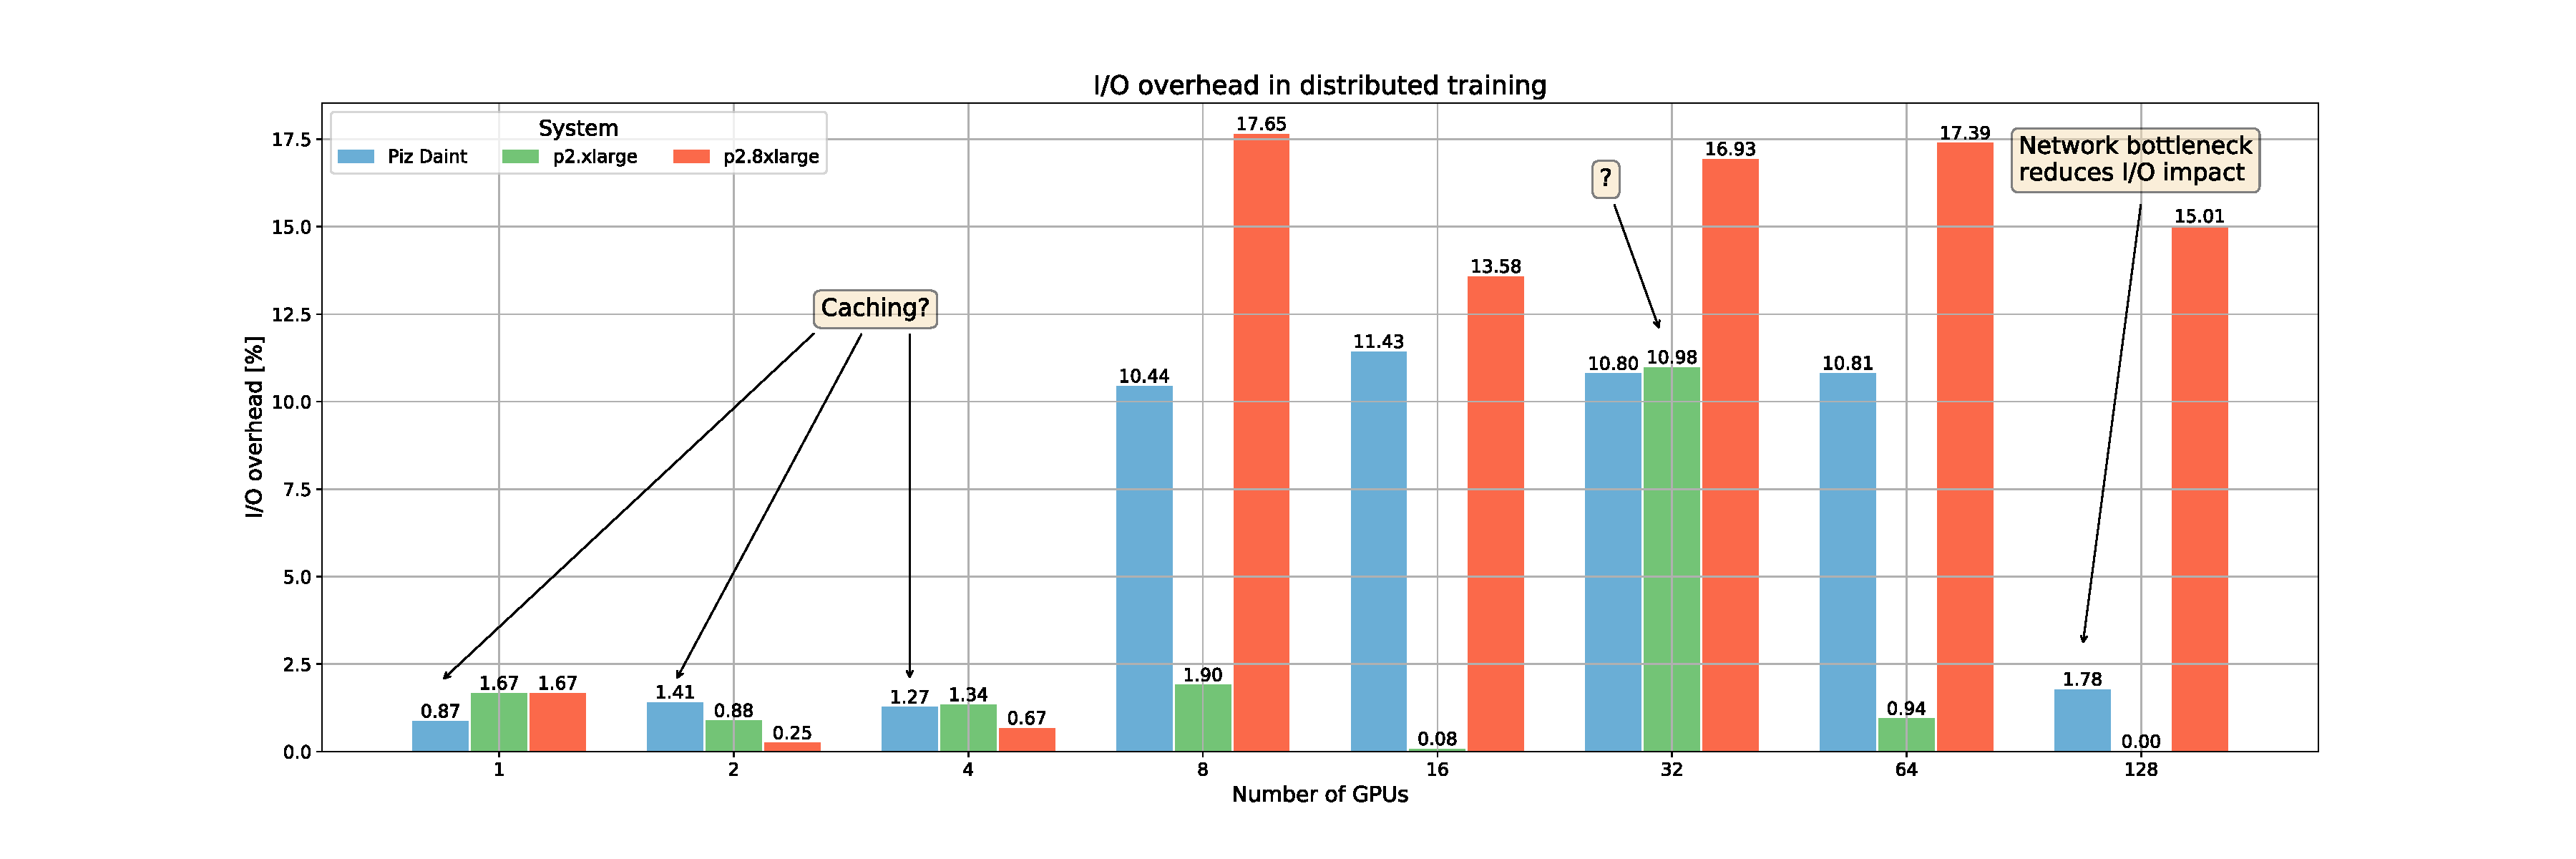
\includegraphics[width=\textwidth,trim={4cm 1.2cm 4.5cm 1.7cm},clip]{io-synthetic-real.pdf}
  \vspace{-0.85cm}
  \caption{I/O overhead in distributed training in terms of number of GPUs for all the systems under study.} 
  \label{fig:io}
\end{figure}
\vspace{-0.5cm}
\newpage

\section{Conclusion and Future Work}
Deep neural networks are being used to solve challenges that not long ago were believed to be infeasible to face.
Deep learning thrives with large neural networks and large datasets, resulting in training times that can be impractical on a single node.\\[-0.4cm]

In this report, we show how to train a model in TensorFlow in a distributed setting and provide benchmarks for InceptionV3 on different systems.\\
The first outcome is that training on eight nodes in Piz Daint achieves close performance to an NVIDIA DGX-1, an integrated system for deep learning.\\
Looking at the scalability on Piz Daint for InceptionV3, we expect an average $11\%$ overhead due to I/O access when compared to the corresponding performance with synthetic data.
Moreover, we expect to detect an inter-node network bottleneck after 64 nodes for this application.\\
In multi-GPU systems, there is no strong dependence on the interconnect up to 16 8-GPU nodes thanks to the local aggregation performed at each node which reduces the inter-node traffic by the number of GPUs per node.
Moreover, using local SSDs and eight GPUs per node adds a constant $17\%$ I/O overhead due to the generated PCIe traffic.\\
Unfortunately, no benchmarks for multiple DGX-1 systems are available at the time of writing, making any direct comparison with Piz Daint impossible.
However, for this application, we expect that it is possible for 64 nodes in Piz Daint to achieve performance close the one of a 8 DGX-1 systems.\\[-0.4cm]

As part of future work, we plan to profile TensorFlow communication patterns to verify our intuition of inter-node network bottleneck when the number of nodes in a systems becomes large.\\
A fundamental topic to be investigated is the resulting training accuracy when an application is trained in multiple single- and multi-GPU systems.
Distributed deep learning is a currentt hot research area. 
Recently, Facebook showed that they trained, with no loss of accuracy, ImageNet in one hour in Caffe2 using ResNet-50~\cite{fair}, while IBM trains ResNet-50 in fifty minutes~\cite{ibm} in Torch in their software-hardware co-optimized distributed deep learning system.\\
Another interesting aspect to look into is how the number of Parameter Servers required to achieve the highest performance for a given number of Workers and nodes depends on the underlying inter-node network capacity.
In fact, both Piz Daint and \textit{p2.xlarge} clusters have single-GPU nodes but when the number of Workers (nodes) becomes large, they require a different number of Parameter Servers to reach their peak performance.
In particular, \textit{p2.xlarge} cluster end up asking for as many Parameter Servers as Workers (we did not test whether more Parameter Servers than Workers might lead to better performance).
\newpage

\bibliographystyle{plain}
\bibliography{biblist}

\end{document}